\documentclass[border=3pt]{standalone}
\usepackage{tikz}
\usepackage{fontspec}
\setmainfont{Myriad Pro}
% set up colour blind friendly palette
\definecolor{cbSkyblue}{RGB}{86,180,233}
\definecolor{cbGreen}{RGB}{0,158,115}
\definecolor{cbYellow}{RGB}{240,228,66}
\definecolor{cbPurple}{RGB}{204,121,167}
\definecolor{monokai}{RGB}{39,40,34}

\begin{document}
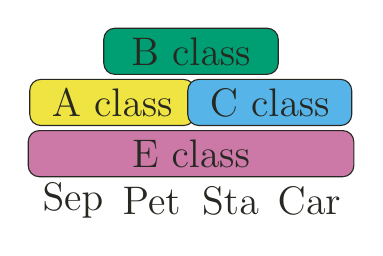
\begin{tikzpicture}
\tikzstyle{every node}=[font=\Large, text=monokai]

  \node[align=center,fill=cbGreen,draw=monokai,rounded corners, inner xsep=10pt] () at (0,1.3) {B class};
  \node[align=center,fill=cbYellow,draw=monokai,rounded corners, inner xsep=8pt] () at (-1,0.65) {A class};
  \node[align=center,fill=cbSkyblue,draw=monokai,rounded corners, inner xsep=8pt] () at (1,0.65) {C class};
  \node[fill=cbPurple,draw=monokai,rounded corners, inner xsep=37.5pt] (flower) at (0,0) {E class};

  \node[] (sepals) at (-1.5,-0.6) {Sep};
  \node[] (petals) at (-0.5,-0.6) {Pet};
  \node[] (stamen) at (0.5,-0.6) {Sta};
  \node[] (carpel) at (1.5,-0.6) {Car};

\end{tikzpicture}
\end{document}
